 Catalyst has a multi-level data architecture, as illustrated in Figure~\ref{fig:db}. 

\begin{figure}[H]
\label{fig:db}
\center{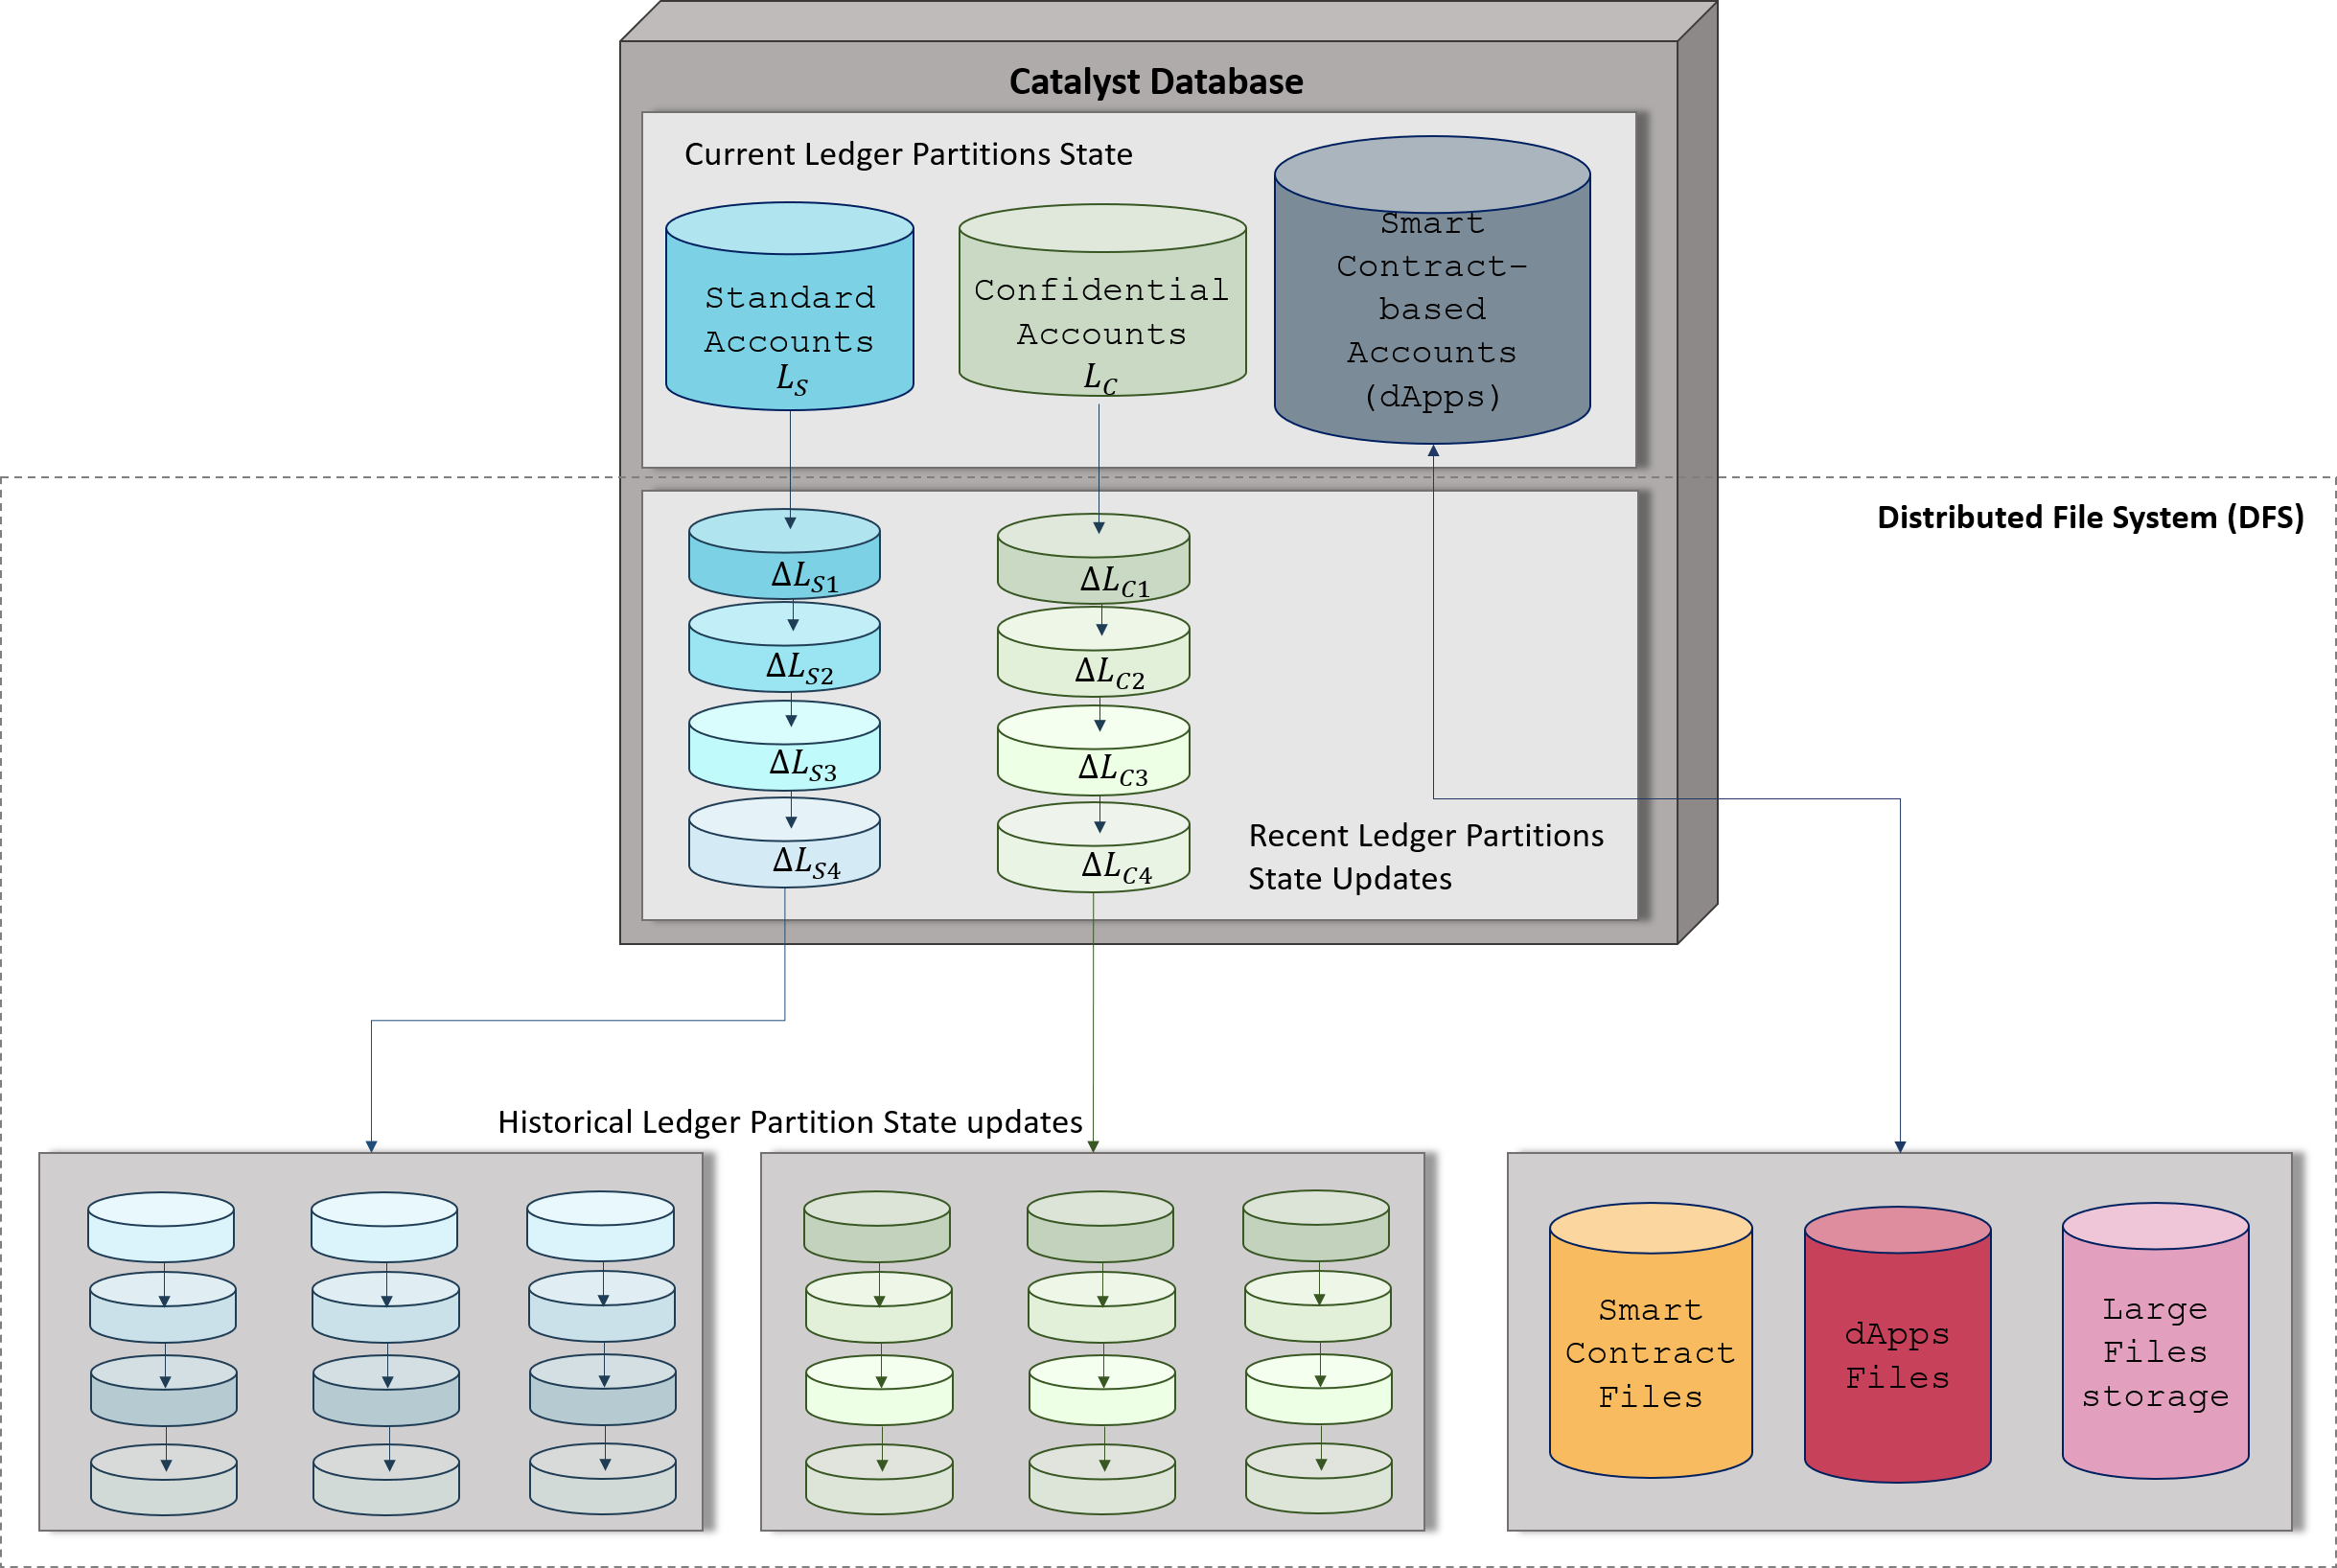
\includegraphics[width=11cm]{Figures/Catalyst_Database}}
\caption{\label{fig:db} Illustration of Catalyst database architecture.}
\end{figure}

At the top level lies the current state of the ledger, \textit{i.e.} the database containing the current balance of digital accounts recorded on the ledger. It represents a snapshot of the ledger state, at the present time. It is periodically updated. At the end of a ledger cycle, that lasts for a fixed period between 30 seconds and 1 minute, a ledger state update is generated by a pool of nodes selected to manage the ledger database, the producers, and distributed to the network users who can then update their local copy of the ledger state. The process followed by producers to generate a ledger update, \textit{i.e.} the consensus-based protocol, is described in section~\ref{Sec:Dem}.\\

The middle level comprises the recent ledger state updates, that is a set of the last recent ledger state updates accepted by producers and broadcast across the network. Historical data, or old ledger state updates, represent the bottom level. Both middle and bottom levels are maintained by the Catalyst Distributed File System (DFS) module. The top and middle levels sits on every node on the network and are thus immediately accessible. On the other hand the bottom level is maintained by some but not necessarily all nodes in the network. Long term data is thus available with a short delay which constitutes a small trade-off for a compact ledger database maintained by every node.\\

Figure~\ref{fig:db} also shows the smart contracts and dApps stored on a database unit separate from the account balances and communicate with DFS for the access, production and storage of files. Technical specificities around smart contracts and dApps are discussed in a paper soon to be released.

